\section{Introduction}
\label{sec:intro}

Multivariate time series data are ubiquitous in our everyday life ranging from the prices in stock markets, the traffic flows on highways, the outputs of solar power plants, the temperatures across different cities, just to name a few. In such applications, users are often interested in the forecasting of the new trends or potential hazardous events based on historical observations on time series signals. For instance, a better route plan could be devised based on the predicted traffic jam patterns a few hours ahead, and a larger profit could be made with the forecasting of the near-future stock market. %Therefore, in this paper, we focus on the multivariate time series forecasting problem, where the difficulties often grow with the length of time series users wish to forecast ahead.

Multivariate time series forecasting often faces a major research challenge, that is, how to capture and leverage the dynamics dependencies among multiple variables.  Specifically,  
%and how to model the  across both time and variables respectively. Firstly, 
real-world applications often entail a mixture of short-term and long-term repeating patterns, as shown in Figure \ref{fig:tra-ex} which plots the hourly occupancy rate of a freeway.
%To illustrate this idea, we plot the hourly occupancy rate of a freeway in Figure \ref{fig:tra-ex}. 
Apparently, there are two repeating patterns, daily and weekly. The former portraits the morning peaks vs. evening peaks, while the latter reflects the workday and weekend patterns. A successful time series forecasting model should be capture both kinds of recurring patterns for accurate predictions. As another example, consider the task of predicting the output of a solar energy farm based on the measured solar radiation by massive sensors over different locations.  The long-term patterns reflect the difference between days vs. nights, summer vs. winter, etc., and the short-term patterns reflect the effects of cloud movements, wind direction changes, etc.  Again, without taking both kinds of recurrent patterns into account, accurate time series forecasting is not possible.  However, traditional approaches such as the large body of work in autoregressive methods \cite{hamilton1994time, box2015time,zhang2003time,Yu_NIPS_16,li2014forecasting} fall short in this aspect, as most of them do not distinguish the two kinds of patterns nor model their interactions explicitly and dynamically. Addressing such limitations of existing methods in time series forecasting is the main focus of this paper, for which we propose a novel framework that takes advantages of recent developments in deep learning research.
%Secondly, there is rich information hidden in the correlation between different variables. For instance, clouds have the most significant influence on the energy output of solar plants. It is plausible to model the relationship between wind directions, the principal factor affecting clouds, and the short-term dependency among the energy output of the solar plants, which is very useful to make accurate forecasts on the future energy productions. Thus how to adequately address the two challenges are essential to develop a reliable multivariate time series forecasting system.
    
    \begin{figure}[!t]
    	\centering
        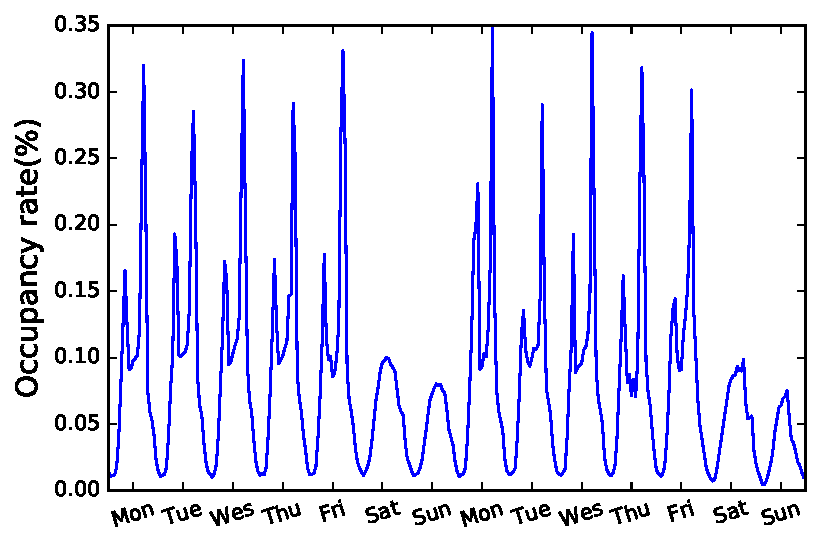
\includegraphics[width=.45\textwidth]{fig/instance.pdf}
        \caption{The hourly occupancy rate of a road in the bay area for 2 weeks}
        \label{fig:tra-ex}
    \end{figure}
    
    \begin{figure*}[!t]
    	\centering
        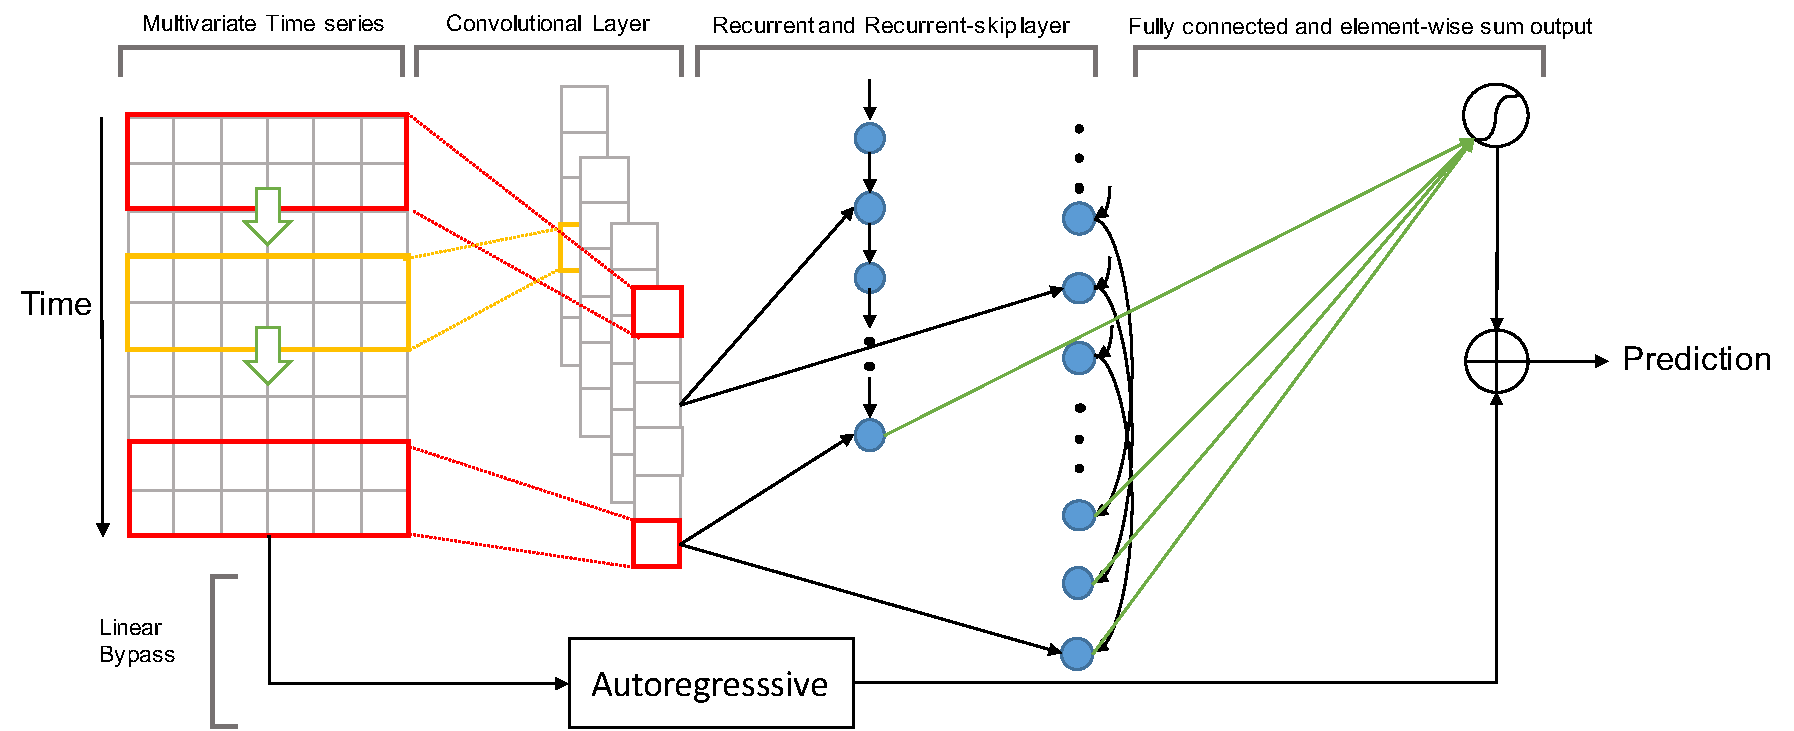
\includegraphics[width=\textwidth]{fig/overview.pdf}
        \caption{An overview of the Long- and Short-term Time-series network (LSTNet)}
        \label{fig:overview}
	\end{figure*}   
    
    Deep neural networks have been intensively studied in related domains, and made extraordinary impacts on the solutions of a broad range of problems.  The recurrent neural networks (RNN) models \cite{elman1990finding}, for example, have become most popular in recent natural language processing (NLP) research.
%to the analysis of sequential data in temporal nature. %\yiming{Hanxiao et al.: How is "sequential data in temporal nature" different from time series data? Your sentence here would confuse (or mislead) readers because it sounds like that RNN has already been intensively studied in time series forecasting.  It follows that our proposed approach is nothing new but incremental. } 
Two variants of RNN in particular, namely the Long Short Term Memory (LSTM) \cite{hochreiter1997long} and the Gated Recurrent Unit (GRU) \cite{chung2014empirical}, have significantly improved the state-of-the-art performance in machine translation, speech recognition and other NLP tasks as they can effectively capture the  meanings of words based on the long-term and short-term dependencies among them in input documents  \cite{bahdanau2014neural,hinton2012deep,krizhevsky2012imagenet}.% where the input can be viewed as discrete data streams. RNNs have an outstanding ability to capture long-term temporal dependencies, a desirable property for multivariate time-series forecasting. 
 In the field of computer vision, as another example, convolution neural network (CNN) models \cite{lecun1995convolutional, krizhevsky2012imagenet} have shown outstanding performance by successfully extracting local and shift-invariant features (called "shapelets" sometimes) at various granularity levels from input images.
%saliences from input signals. CNNs are designed for introducing locality to the patterns matched in input data and to enable translational invariance with respect to the exact location, which is the timestamp in time series data. The need of automatically capturing those salient features, or ``shapelets'' over time, makes CNNs suitable for detecting locality patterns in multivariate time series data. 
    
Deep neural networks have also received an increasing amount of attention in time series analysis. A substantial portion of the previous work has been focusing on \textit{time series classification}, i.e., the task of automated assignment of class labels to time series input. For instance, RNN architectures have been studied for extracting informative patterns from health-care sequential data \cite{lipton2015learning,che2016recurrent} and classifying the data with respect diagnostic categories.  RNN has also been applied to mobile data, for classifying the input sequences with respect to actions or activities \cite{hammerla2016deep}. CNN models have also been used in action/activity recognition \cite{lea2016temporal,yang2015deep,hammerla2016deep}, for the extraction of shift-invariant local patterns from input sequences as the features of classification models.

Deep neural networks have also been studied for \textit{time series forecasting}, i.e., the task of using observed time series in the past to predict the unknown time series in a look-ahead horizon -- the larger the horizon, the harder the problem. Efforts in this direction range from the early work using naive RNN models \cite{connor1991recurrent} and the hybrid models \cite{zhang1998forecasting,zhang2003time,jain2007hybrid} combining the use of ARIMA \cite{box1970distribution} and Multilayer Perceptron (MLP), to the recent combination of vanilla RNN and Dynamic Boltzmann Machines in time series forecasting \cite{dasgupta2016nonlinear}.

Although the aforementioned work have shed lights on how to use  deep neural networks to improve time series analysis, none of them has offered good answers for the important questions below:
\begin{itemize}
 \item How can RNN (LSTM and GRU) and CNN be effectively combined for dynamic modeling of short-term and long-term dependency patterns in multi-variate time series data?
 \item How much can the combined deep learning approach (CNN + RNN) improve the performance of representative autoregressive models? 
 \item Can we further combine the deep learning models (CNN + RNN) and traditional autoregressive models to achieve better performance than that of using each type of the models alone?
\end{itemize}  


%However, to the best of our knowledge, no work has been conducted to examine how to utilize the RNN(LSTM and GRU) and CNN structures efficiently in the task of multivariate time series forecasting or compare it with the classical time series models.

%\yiming{If you want, you may use the following paragraph in the empirical results analysis part of the paper, but not here.}

%In contrast, traditional time series forecasting models cannot well handle long-term dependencies. Increasing the input window size will cause severer over-fitting due to the substantially increased number of parameters. This is not the case for RNNs and CNNs whose number of parameters remain constant as the length of input sequence increases. In addition, traditional approaches usually assume a consistent variables relationship across the whole time dimension, e.g the commonly used vector autoregressive model. However, time series data often exhibits different variable dependency patterns at different time stamps, possibly due the influence of underlying hidden factors. Following this intuition, the CNN structure is naturally suitable for discovering \emph{multiple} local variables relationship in a data-driven manner.
%   In this paper, 
Answering the above questions are crucial for improving the state-of-the-art in time series forecasting, and is the main contribution we aim in this paper.  Specifically, we propose a novel deep learning framework, namely Long- and Short-term Time-series Network (LSTNet), as illustrated in Figure \ref{fig:overview}. It leverages the strengths of both the convolutional layer to discover the local dependency patterns among multi-dimensional input variables, and the recurrent layer that captures complex long-term dependencies. A particular recurrent structure, namely Recurrent-skip, is designed for capturing very long-term dependence patterns and making the optimization easier as it utilizes the periodic property of the input time series signals. Finally, the LSTNet incorporates a traditional autoregressive linear model in parallel to the non-linear neural network part; which is similar to a \textit{highway component} \cite{srivastava2015highway}. Adding the linear model to this framework we aim to address a potential weakness of the neural-network model, i.e., when/if the non-linear model is not sufficiently sensitive to the scale changes in input data, the linear model provides a better (more sensitive) alternative. Our evaluation results (Section \ref{sec:ablation}) provide empirical evidence for this assertion. 
% The linear model is sensitive to the scale changing of time series data, which is crucial to some forecasting tasks. To achieve that, we use an autoregressive model as a highway component \cite{srivastava2015highway}. 
%In our experiments on multiple real-world datasets, the proposed method (LSTNet) consistently outperformed other state-of-the-art methods. 
% We also provide a careful ablation study to justify the effectiveness of different components of our deep learning framework for multivariate time series forecasting.
     
     The rest of this paper is organized as follows. Section \ref{sec:related} outlines the related background, including representative auto-regressive methods and Gaussian Process models. Section \ref{sec:model} describe our proposed LSTNet. Section \ref{sec:experiment} reports the evaluation results of our model in comparison with strong baselines on real-world datasets. Finally, we conclude our findings in Section \ref{sec:conclusion}.
       
     